\documentclass{beamer}

\usepackage{beamerthemesplit}
\usetheme{Singapore} %Copenhagen}
%\usecolortheme{whale}

\beamertemplatenavigationsymbolsempty % Hide navigation panel

\usepackage[T2A]{fontenc}
\usepackage[utf8]{inputenc}
\usepackage[russian]{babel}


\usepackage{textcomp}
\usepackage{amssymb,amsmath}
%\usepackage{animate}
%\usepackage{longtable}
\usepackage{xcolor}

%\usepackage{pstricks}

\newcounter{N}

%% Форматирование окружения itemize
%\usepackage{ragged2e}
%\let\olditem\item
%\renewcommand\item{\olditem\justifying}


\title[]{Дифференциальные операторы в криволинейной системе координат}

\author[]{ {\em Верещагин Антон Сергеевич}
	\\
	канд. физ.-мат. наук, доцент\\
	\bigskip
	Кафедра аэрогидродинамики ФЛА НГТУ
}

\newtheorem{dfn}{Определение}  
\newtheorem{theorems}{Теорема}  

\newcommand{\Rn}{\mathrm{R}^n}
\newcommand{\Sm}{\mathrm{S}^m}
\newcommand{\Ql}{\mathrm{Q}^l}

\newcommand{\Rd}[1]{\mathbb{R}^{#1}}
\newcommand{\Vn}{\mathrm{V}^n}

\newcommand{\oper}[1]{{\bf #1}}
\newcommand{\basis}[1]{\vec{\bf #1}}
\newcommand{\dt}[1]{\frac{d #1}{dt}}
\newcommand{\dtds}[1]{\displaystyle\frac{d #1}{dt}}
\newcommand{\ds}[1]{\frac{d #1}{ds}}
\newcommand{\dsds}[1]{\displaystyle\frac{d #1}{ds}}
\newcommand{\dsd}[1]{\frac{d^2 #1}{ds^2}}
\newcommand{\pdt}[1]{\frac{\partial #1}{\partial t}}
\newcommand{\pds}[1]{\frac{\partial #1}{\partial s}}
\newcommand{\pdx}[1]{\frac{\partial #1}{\partial x}}
\newcommand{\pdy}[1]{\frac{\partial #1}{\partial y}}
\newcommand{\pdz}[1]{\frac{\partial #1}{\partial z}}
\newcommand{\pdxds}[1]{\displaystyle\frac{\partial #1}{\partial x}}
\newcommand{\pdyds}[1]{\displaystyle\frac{\partial #1}{\partial y}}
\newcommand{\pdzds}[1]{\displaystyle\frac{\partial #1}{\partial z}}
\newcommand{\pdn}[1]{\frac{\partial #1}{\partial n}}
\newcommand{\grad}[1]{\operatorname{grad} #1}
\newcommand{\gradv}[1]{\basis{i}\pdx{#1}+\basis{j}\pdy{#1}+\basis{k}\pdz{#1}}
\newcommand{\gradvds}[1]{\basis{i}\pdxds{#1}+\basis{j}\pdyds{#1}+\basis{k}\pdzds{#1}}

\newcommand{\pd}[2]{\frac{\partial #1}{\partial #2}}

\newcommand{\pdxt}[1]{\frac{\partial^2 #1}{\partial x^2}}
\newcommand{\pdyt}[1]{\frac{\partial^2 #1}{\partial y^2}}
\newcommand{\pdzt}[1]{\frac{\partial^2 #1}{\partial z^2}}


\newcommand{\dv}[1]{\operatorname{div}\vec{#1}}
\newcommand{\dvdef}[1]{\pdx{#1_x}+\pdy{#1_y}+\pdz{#1_z}}
\newcommand{\dvdefds}[1]{\pdxds{#1_x}+\pdyds{#1_y}+\pdzds{#1_z}}
\newcommand{\dvwv}[1]{\operatorname{div} #1}
\newcommand{\rot}[1]{\operatorname{rot}\vec{#1}}
\newcommand{\rotpr}[2]{\operatorname{rot}_{#1}\vec{#2}}
\newcommand{\rotwv}[1]{\operatorname{rot} #1}

\newcommand{\lapl}[1]{\pdxt{#1}+\pdyt{#1}+\pdzt{#1}}

\newcommand{\argq}{(q_1,q_2,q_3)}
\newcommand{\argx}{(x,y,z)}


\begin{document}

\frame{\titlepage}


\frame{
\frametitle{Аннотация}
\parbox{\textwidth}{
Криволинейные координаты. Коэффициенты Ляме. Дифференциальные операторы в криволинейных координатах.
}
}

\frame{
\frametitle{Криволинейные системы координат}
\begin{dfn}
\parbox{\textwidth}{
Три скалярные величины ($q_1$, $ q_2 $, $ q_3 $), однозначно определяющие точку в пространстве, называются \alert{криволинейными координатами точки}. \pause 
}
\end{dfn}

\medskip
\parbox{\textwidth}{
Пусть в декартовой системе координат точка имеет координаты $(x,y,z)$, тогда существует взаимнооднозначное отображение, связывающее различные системы координат: \pause 
\begin{columns}
\begin{column}{0.4\textwidth}
\[
\left\{
\begin{array}{rcl}
x & = & x\argq, \\
y & = & y\argq, \\
z & = & z\argq
\end{array}
\right.
\] \pause 
\end{column}
\begin{column}{0.2\textwidth}
и наоборот
\end{column}
\begin{column}{0.4\textwidth}
\[
\left\{
\begin{array}{rcl}
q_1 & = & q_1\argx, \\
q_2 & = & q_2\argx,\\
q_3 & = & q_3\argx.
\end{array}
\right.
\]
\end{column}
\end{columns}


}

}


\frame{
\frametitle{Линии и поверхности уровня}
\begin{dfn}
\parbox{\textwidth}{
Линии $q_1={\rm const}$, $q_2={\rm const}$, $q_3={\rm const}$ называются \alert{поверхностями уровня} или \alert{координатными поверхностями}.  \pause А линии пересечения двух таких поверхностей называются \alert{координатными линиями}. \pause 
}
\end{dfn}

\begin{exampleblock}{Цилиндрическая система координат}
\begin{columns}
\begin{column}{0.3\textwidth}
\[
\left\{
\begin{array}{rcl}
x & = & r \cos \varphi, \\
y & = & r \sin \varphi, \\
z & = & z.
\end{array}
\right.
\] \pause 
\[
\left\{
\begin{array}{rcl}
r & = & \sqrt{x^2+y^2}, \\
\varphi & = & \arctan{y/x},\\
z & = & z.
\end{array}\right.
\] \pause 
\end{column}
\begin{column}{0.7\textwidth}
\centering 
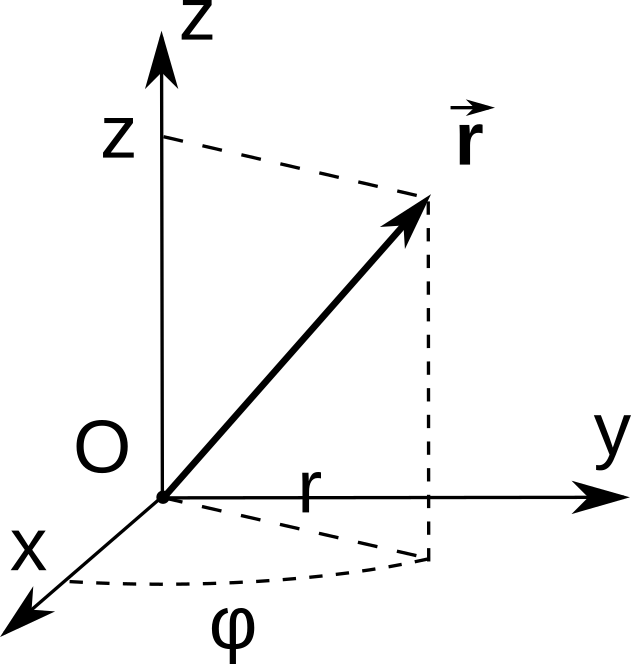
\includegraphics[width=0.5\textwidth]{../img/cylindr.png}
\end{column}
\end{columns}
\end{exampleblock}
}


\frame{
\frametitle{Координатные линии и координатные поверхности в цилиндрической системе координат}
\centering
\begin{tabular}{c|c|c}
$r=const$ & $\varphi=const$ & $ z=const$ \\
& & \\
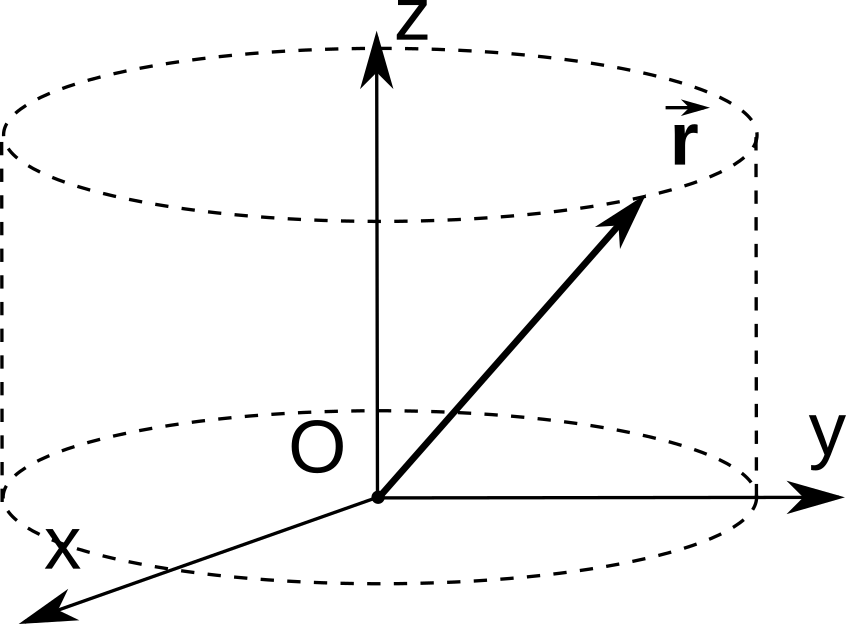
\includegraphics[width=0.3\textwidth]{../img/cylindr_iso_r.png}  \pause & 
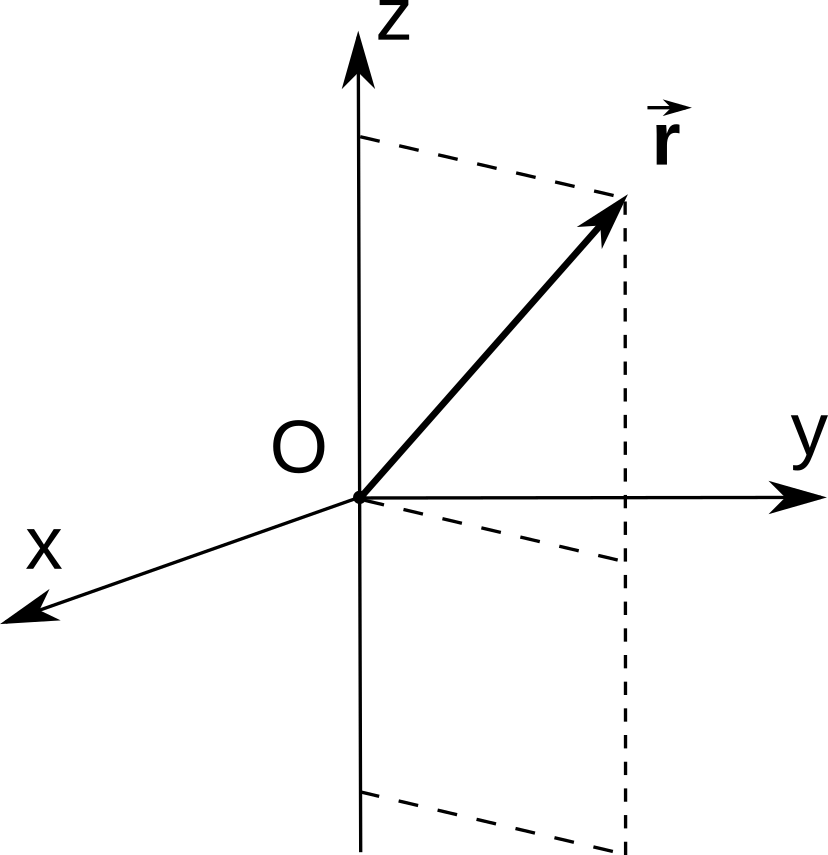
\includegraphics[width=0.3\textwidth]{../img/cylindr_iso_phi.png} \pause & 
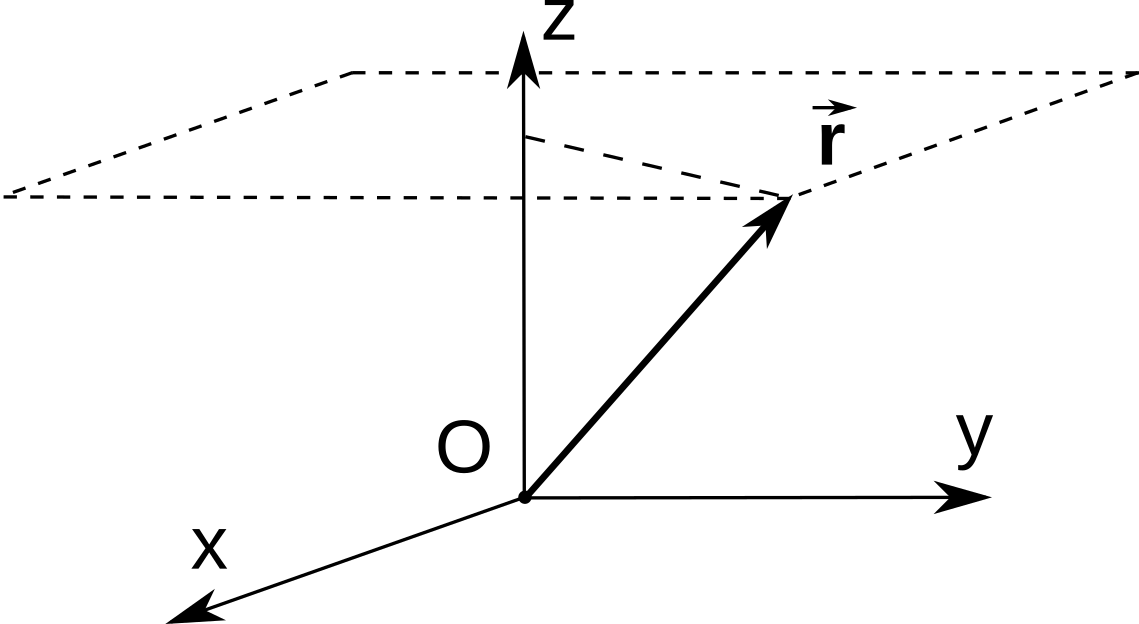
\includegraphics[width=0.35\textwidth]{../img/cylindr_iso_z.png}
\end{tabular}

}


\frame{
\frametitle{Коэффициенты Ляме}
\begin{columns}
\begin{column}{0.4\textwidth}
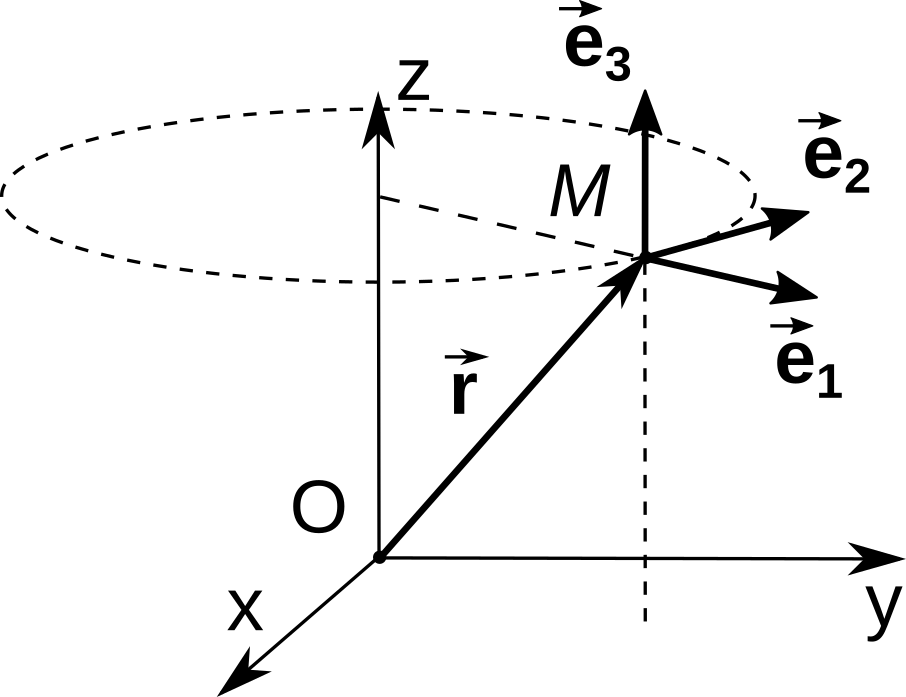
\includegraphics[width=\textwidth]{../img/lame.png} \pause 
\end{column}
\begin{column}{0.6\textwidth}
\parbox{\textwidth}{
Рассмотрим фиксированную точку $ M $, и введем единичные векторы 
\[
\begin{array}{c}
\vec{e}_1,\quad
\vec{e}_2,\quad
\vec{e}_3\\
(||\vec{e}_1||=||\vec{e}_2||=||\vec{e}_3||=1),
\end{array}
\]
направленные вдоль касательных к координатным линиям в сторону возрастания координат.
} \pause 
\end{column}
\end{columns}
\parbox{\textwidth}{
Пусть 
\[
\vec{r}=x\argq\basis{i}+y\argq\basis{j}+z\argq\basis{k}, \pause 
\]
тогда рассмотрим
\[
\pd{\vec{r}}{q_1}=\pd{x}{q_1}\basis{i}+\pd{y}{q_1}\basis{j}+\pd{z}{q_1}\basis{k} = \pause 
H_1\vec{e}_1,\quad H_1=\left|\pd{\vec{r}}{q_1}\right|.
\]
}
}

\frame{
\frametitle{Коэффициенты Ляме}
\parbox{\textwidth}{
Общие формулы
\[
\pd{\vec{r}}{q_i}=H_i\vec{e}_i,\quad 
H_i^2=\left(\pd{x}{q_i}\right)^2+\left(\pd{y}{q_i}\right)^2+\left(\pd{z}{q_i}\right)^2 \quad 
(i=1,2,3).
\] \pause 


\begin{dfn}
Величины $H_i$ $(i=1,2,3)$ называются \alert{коэффициентами Ляме}.
\end{dfn}
}

}

\frame{
\frametitle{Коэффициенты Ляме для цилиндрической системы координат}

\begin{columns}
\begin{column}{0.4\textwidth}
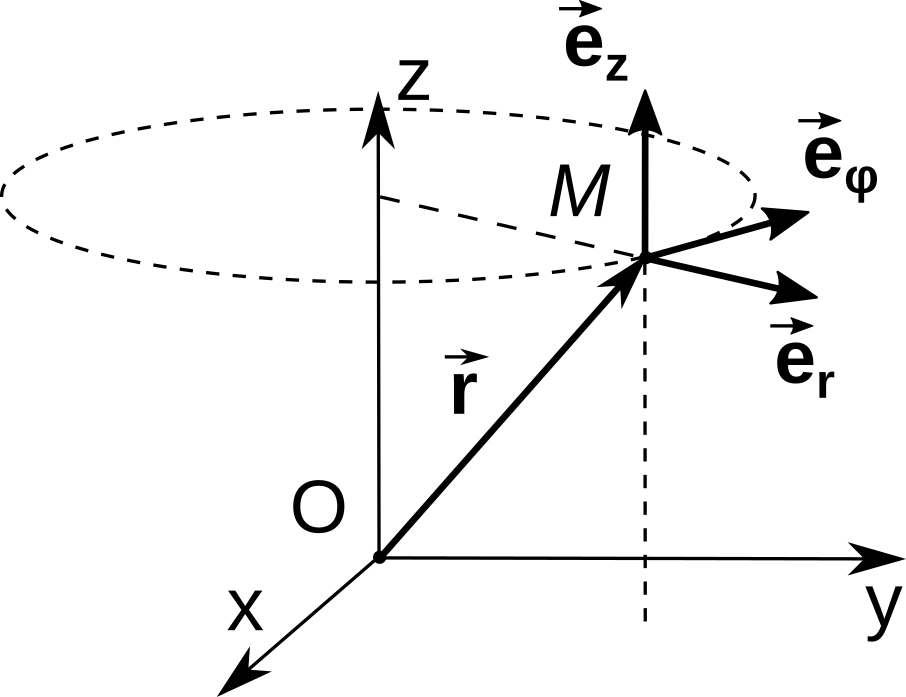
\includegraphics[width=\textwidth]{../img/lame_example.png} \pause 
\[
\left\{
\begin{array}{rcl}
x & = & r \cos \varphi, \\
y & = & r \sin \varphi, \\
z & = & z.
\end{array}
\right.
\] \pause 
\end{column}
\begin{column}{0.7\textwidth}
\[
\begin{array}{l}
H_r = \displaystyle\sqrt{\left(\pd{x}{r}\right)^2+\left(\pd{y}{r}\right)^2+\left(\pd{z}{r}\right)^2}=1,\\ \pause 
H_{\varphi} = \displaystyle\sqrt{\left(\pd{x}{\varphi}\right)^2+\left(\pd{y}{\varphi}\right)^2+\left(\pd{z}{\varphi}\right)^2}=r,\\ \pause 
H_{z} = \displaystyle\sqrt{\left(\pd{x}{z}\right)^2+\left(\pd{y}{z}\right)^2+\left(\pd{z}{z}\right)^2}
=1. \pause 
\end{array}
\]

\end{column}
\end{columns}

\medskip
\parbox{\textwidth}{
Из построения векторов $\vec{e}_r$, $\vec{e}_{\varphi}$ и $\vec{e}_z$ видно, что они \alert{взаимно ортогональны}.
}
}


\frame{
\frametitle{Предположение об ортогональности криволинейной системы координат}

\parbox{\textwidth}{
Далее будем рассматривать только \alert{ортогональные криволинейные системы координат}:
\[
\vec{e}_i\cdot\vec{e}_j=\delta_{ij}=
\left\{
\begin{array}{ll}
1, & i=j,\\
0, & i\neq j,
\end{array}
\right.
\]
\[
(i,j=1,2,3).
\] \pause 

\medskip
$\delta_{ij}$ называется \alert{символом Кронекера}.
}

}


\frame{
\frametitle{Градиент в криволинейной системе координат}
Из выражений
\begin{equation}
\label{eq:dq}
dq_i=\grad{q_i}\cdot d\vec{r}\quad
(i=1,2,3)
\end{equation} \pause 
и 
\begin{equation}
\label{eq:dr}
d\vec{r}=\pd{\vec{r}}{q_1}dq_1+\pd{\vec{r}}{q_2}dq_2+\pd{\vec{r}}{q_3}dq_3
\end{equation} \pause 
подстановкой (\ref{eq:dr}) в (\ref{eq:dq}) при $i=1$ получим
\[
dq_1=\grad{q_1}\cdot \left(\pd{\vec{r}}{q_1}dq_1+\pd{\vec{r}}{q_2}dq_2+\pd{\vec{r}}{q_3}dq_3\right)
\] \pause 
\[
0=\left(\grad{q_1}\cdot \pd{\vec{r}}{q_1}-1\right) dq_1+\left(\grad{q_1}\cdot\pd{\vec{r}}{q_2}\right) dq_2+\left(\grad{q_1}\cdot\pd{\vec{r}}{q_3}\right) dq_3
\] \pause 
В силу произвольности $dq_i$ ($i=1,2,3$)
\[
\grad{q_1}\cdot \pd{\vec{r}}{q_1} = 1,\quad
\grad{q_1}\cdot\pd{\vec{r}}{q_2} = 0,\quad
\grad{q_1}\cdot\pd{\vec{r}}{q_3} = 0.
\]
}

\frame{
\frametitle{Градиент в криволинейной системе координат}
\[
\grad{q_1}\cdot \pd{\vec{r}}{q_1} = 1,\quad
\grad{q_1}\cdot\pd{\vec{r}}{q_2} = 0,\quad
\grad{q_1}\cdot\pd{\vec{r}}{q_3} = 0.
\] \pause 

Т.к. $\displaystyle\pd{\vec{r}}{q_i} = H_i\vec{e}_i$ и $\vec{e}_i$ ($i=1,2,3$) взаимноортогональны,  \pause тогда
\[
\grad{q_1}=\frac{1}{H_1}\vec{e}_1.
\] \pause 

Повторяя проделанную процедуру для $i=2,3$, получим что
\[ 
\grad{q_i}=\frac{1}{H_i}\vec{e}_i\quad (i=1,2,3).
\]
}

\frame{
\frametitle{Градиент в криволинейной системе координат}


Воспользуемся для разложения градиента
\[
\grad{\varphi(q_1,q_2,q_3)}=\pd{\varphi}{q_1}\grad{q_1}+\pd{\varphi}{q_2}\grad{q_2}+\pd{\varphi}{q_3}\grad{q_3}.
\] \pause 


И тогда
\[ 
\grad{\varphi}=\frac{\vec{e}_1}{H_1}\pd{\varphi}{q_1}+\frac{\vec{e}_2}{H_2}\pd{\varphi}{q_2}+\frac{\vec{e}_3}{H_3}\pd{\varphi}{q_3}.
\]
}

\frame{
\frametitle{Криволинейные составляющие вектора}
\parbox{\textwidth}{
В локальной системе координат произвольный вектор можно разложить по базису
\[ 
\vec{a}=a_1\vec{e}_1+a_2\vec{e}_2+a_3\vec{e}_3.
\]
Скалярные величины $ a_i $ ($i=1,2,3$) называются \alert{криволинейными составляющими вектора} $ \vec{a} $.
}
}

\frame{
\frametitle{Элементарный параллелепипед}


\centering
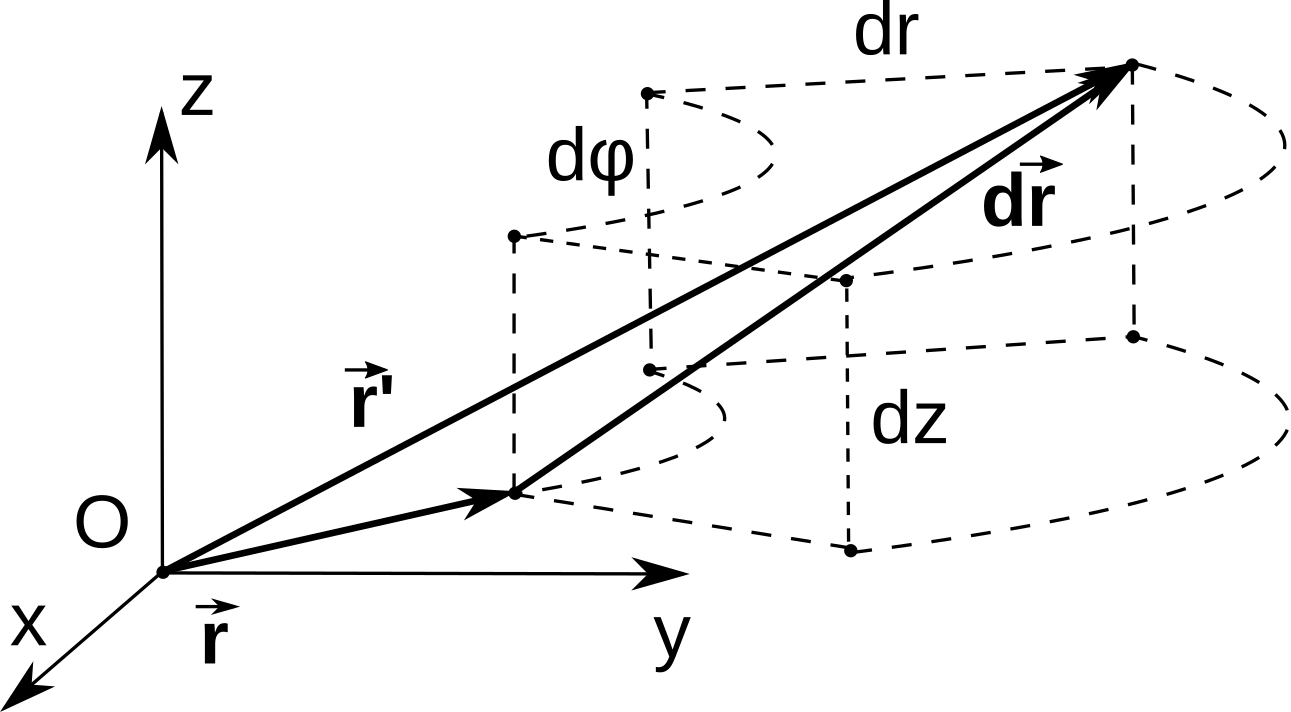
\includegraphics[width=0.9\textwidth]{../img/elem_paral_dq.png} \pause 

\[ 
d\vec{r}=\pd{\vec{r}}{q_1}dq_1+\pd{\vec{r}}{q_2}dq_2+\pd{\vec{r}}{q_3}dq_3=H_1dq_1\vec{e}_1+H_2dq_2\vec{e}_2+H_3dq_3\vec{e}_3.
\]

}

\frame{
\frametitle{Длины сторон элементарного параллелепипеда}
\begin{center}
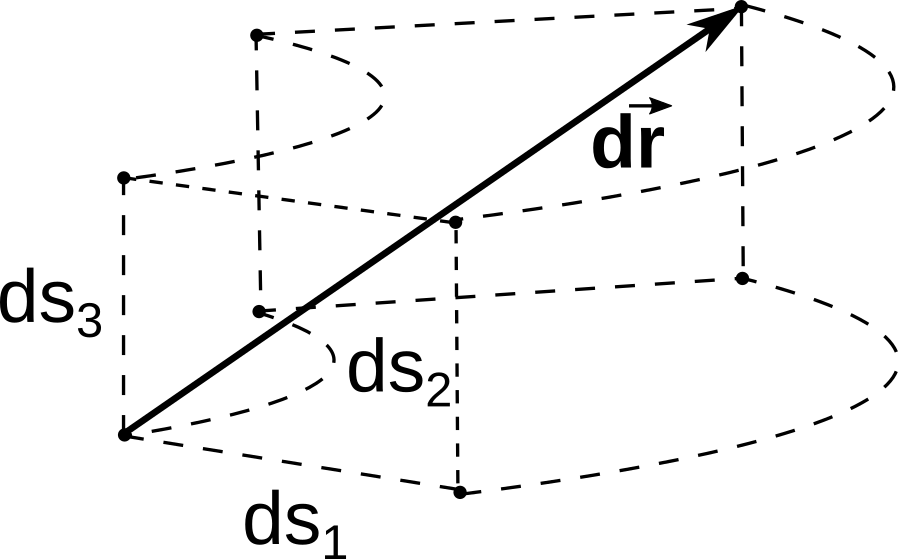
\includegraphics[width=0.5\textwidth]{../img/elem_paral_ds.png}
\end{center} \pause 
Отсюда составляющие длины
\[
ds_i=H_idq_i \quad (i=1,2,3).
\] \pause 
и
\[ 
ds^2=H_1^2dq_1^2+H_2^2dq_2^2+H_3^2dq_3^2.
\] \pause 
Объем элементарного параллелепипеда
\[
dV = H_1 H_2 H_3 dq_1 dq_2 dq_3.
\]
} 

\frame{
\frametitle{Дивергенция в криволинейной системе координат}

\begin{columns}
\begin{column}{0.5\textwidth}
\centering
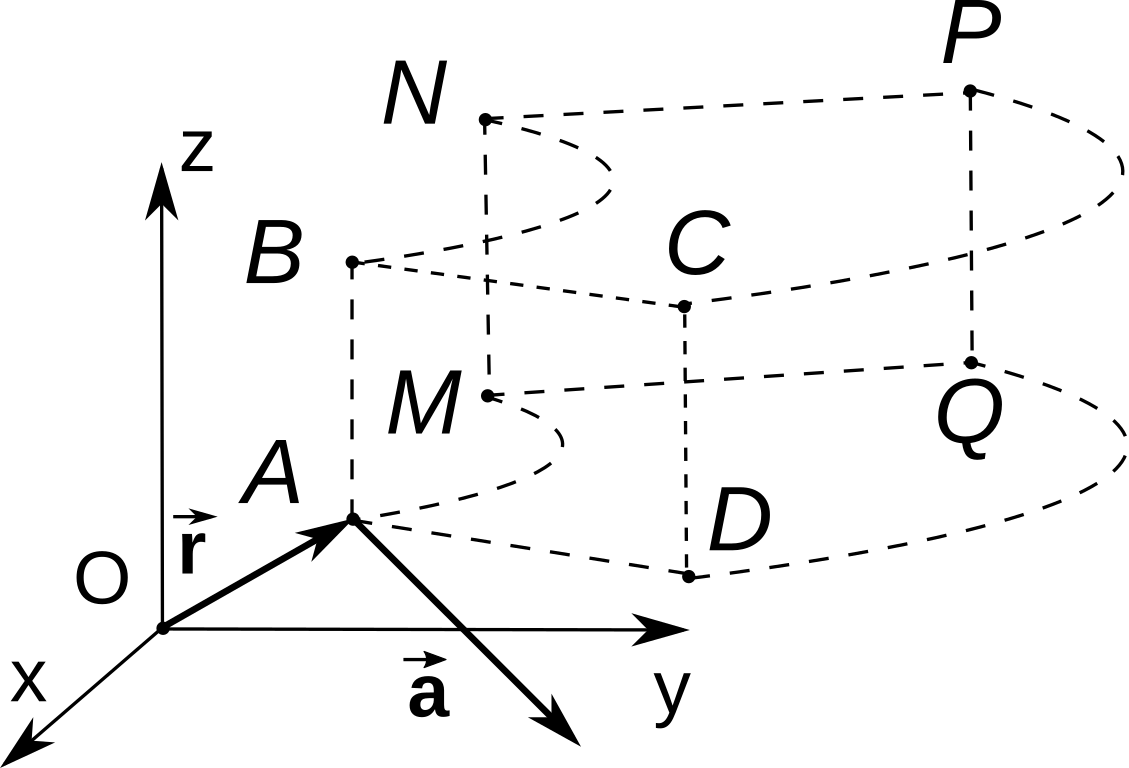
\includegraphics[width=\textwidth]{../img/elem_paral.png}
\end{column}
\begin{column}{0.5\textwidth}
\parbox{\textwidth}{
\[
\dv{a}=\lim_{V\to 0}\frac{\int\limits_S \vec{a}\cdot\vec{n}dS}{V},
\]
где $\vec{a}$ -- заданное векторное поле; $\vec{n}$ -- вектор внешней единичной нормали; $S$ -- площадь поверхности объема $V$.
}
\end{column}
\end{columns}
\begin{center}

\parbox{\textwidth}{
\only<1>{
Для элементарного параллелепипеда $ABCDMNPQ$
\[
\dv{a}=\frac{\vec{a}\cdot\vec{n}_{ABCD}S_{ABCD}+\ldots}{V_{ABCDPQNM}}.
\]
}
\only<2>{
Потоки векторов через элементарные площадки равны
\[
\begin{array}{c}
\vec{a}\cdot\vec{n}_{ABCD}S_{ABCD}=-a_2 ds_1 ds_3=-a_2 H_1 H_3 dq_1 dq_3,\\
\vec{a}\cdot\vec{n}_{AMNB}S_{AMNB}=-a_1 ds_2 ds_3=-a_1 H_2 H_3 dq_2 dq_3,\\
\vec{a}\cdot\vec{n}_{AMQD}S_{AMQD}=-a_3 ds_1 ds_2=-a_3 H_1 H_2 dq_1 dq_2,
\end{array}
\]
}

\only<3>{
Потоки векторов через элементарные площадки равны
\[
\begin{array}{l}
\vec{a}\cdot\vec{n}_{MNPQ}S_{MNPQ}=\displaystyle(a_2H_1 H_3 + \pd{a_2 H_1 H_3}{q_2}dq_2) dq_1 dq_3,\\
\vec{a}\cdot\vec{n}_{DCPQ}S_{DCPQ}=\displaystyle(a_1H_2 H_3 + \pd{a_1H_2 H_3}{q_1}dq_1)dq_2 dq_3,\\
\vec{a}\cdot\vec{n}_{BNPC}S_{BNPC}=\displaystyle(a_3H_1 H_2  + \pd{a_3H_1 H_2}{q_3}dq_3)dq_1 dq_2.
\end{array}
\]
}

\only<4>{
\[
\begin{array}{c}

\dv{a}=\displaystyle\frac{(\vec{a}\cdot\vec{n}_{ABCD}S_{ABCD}+\vec{a}\cdot\vec{n}_{MNPQ}S_{MNPQ})+\ldots}{V_{ABCDPQNM}}=\\
=\displaystyle\frac{\displaystyle\pd{a_2H_1 H_3}{q_2}dq_2  dq_1 dq_3+
\pd{a_1H_2 H_3}{q_1}dq_1  dq_2 dq_3+
\pd{a_3H_1 H_2}{q_3}dq_3  dq_1 dq_2}{H_1 H_2 H_3 dq_1 dq_2 dq_3}=\\
=\displaystyle\frac{1}{H_1H_2H_3}\left(
\pd{(H_2 H_3a_1)}{q_1} +
\pd{(H_1 H_3a_2)}{q_2} +
\pd{(H_1 H_2a_3)}{q_3} 
\right).
\end{array}
\]

}
}

\end{center}


}

\end{document}

